% !TEX root = ../main.tex

\chapter{蛋白质功能预测的相关研究概述}

\section{引言}

蛋白质功能预测是生物信息学中的重要研究任务，其核心目标是利用计算方法为尚未充分注释的蛋白质自动赋予功能标签。实现这一目标既需要合理的计算建模方法，也离不开生物学背景知识的支撑。本章为后续方法设计中的问题定义、评价体系、零样本学习框架和预训练技术选型提供必要的前序知识与理论基础。

本章的组织结构如下：2.2节介绍蛋白质功能预测问题的定义与常用评价指标；2.3节介绍零样本学习的形式化定义、嵌入空间对齐机制与基于对比学习的语义匹配方法；2.4节系统介绍预训练技术的基本原理，涵盖语言模型预训练、蛋白质语言模型、多模态预训练、参数高效微调与知识蒸馏等关键方向；2.5节对本章内容进行总结。

\section{蛋白质功能预测问题}

\subsection{蛋白质功能预测问题的定义}

蛋白质功能预测通常以基因本体（Gene Ontology, GO）\cite{ashburner2000gene}作为标准化注释体系。GO将蛋白质功能划分为生物过程（Biological Process, BP）、分子功能（Molecular Function, MF）和细胞组分（Cellular Component, CC）三个相互独立但内部结构复杂的子本体。每个GO术语不仅具有标准化名称和文本定义，还通过``is\_a''和``part\_of''等关系组织成有向无环图（Directed Acyclic Graph, DAG）\cite{goeman2008multiple}，子节点是父节点的具体化，如图~\ref{fig:go_dag}所示。这种层级结构使蛋白质功能预测区别于普通的多标签分类任务：不同标签之间存在明确的祖先—后代依赖关系，且越接近叶节点的术语语义越具体、样本越稀疏。

\begin{figure}[htbp]
\centering
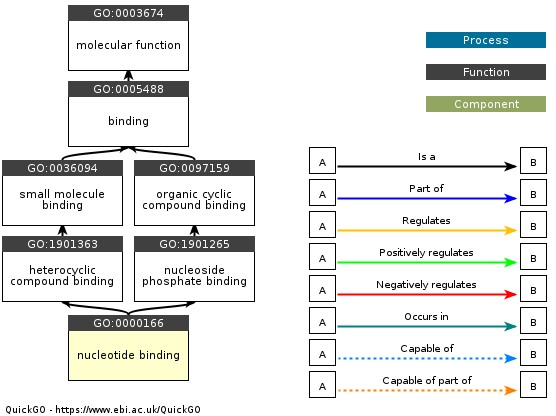
\includegraphics[width=1.0\textwidth]{figures/go_structure.jpg}
\caption{GO树状层级结构示例}
\label{fig:go_dag}
\end{figure}

在GO体系下，蛋白质功能预测通常被形式化为多标签分类问题。设蛋白质集合$\mathcal{P}=\{P_1,P_2,\ldots,P_N\}$包含$N$个蛋白质，$\mathcal{X} = \{X_1, X_2, \ldots, X_N\}$为对应的特征向量，这些特征既可来自单一数据源，也可由多种数据源联合提取。某一GO子本体对应的候选功能术语集合记为$\mathcal{G} = \{g_1, g_2, \ldots, g_C\}$，其中$C$为该子本体中候选GO术语的总数。蛋白质$P_i$的功能注释可表示为如公式~\eqref{eq:go_annotation}所示的二元向量：
\begin{equation}
\label{eq:go_annotation}
\mathbf{y}_i \in \{0,1\}^C, \quad y_{ic} =
\begin{cases}
1 & \text{当蛋白质}P_i\text{具有功能}g_c \\
0 & \text{否则}
\end{cases}
\end{equation}
给定训练集$\mathcal{D} = \{(P_i, \mathbf{y}_i)\}_{i=1}^{N}$，学习映射函数$f_\theta: \mathcal{X} \to [0,1]^C$，通过最小化如公式~\eqref{eq:multilabel_loss}所示的多标签损失函数优化参数：
\begin{equation}
\label{eq:multilabel_loss}
\mathcal{L}(\theta) = -\sum_{i=1}^{N}\sum_{c=1}^{C}\left[y_{ic}\log f_\theta(P_i)_c + (1-y_{ic})\log(1-f_\theta(P_i)_c)\right]
\end{equation}

值得注意的是，GO标签满足真实路径规则（True Path Rule）：若蛋白质被标注了某个GO术语，则其也应具有该术语所有祖先节点所代表的更一般功能。这意味着训练数据和评估标签通常需要进行向上传播以避免标签不一致问题，同时要求模型在预测时不仅判断单一标签是否成立，还需兼顾标签之间的层级一致性。

除封闭标签空间下的多标签分类建模外，近年来越来越多的研究将蛋白质功能预测重新定义为"蛋白质—功能标签"匹配问题。设$P$表示蛋白质输入，$g_c$表示第$c$个GO术语的文本定义或语义表示，则模型可以直接学习二者之间的匹配分数，如公式~\eqref{eq:matching_score}所示：
\begin{equation}
\label{eq:matching_score}
s(P, g_c) = p(y=1 \mid P, g_c)
\end{equation}
这种建模方式能够自然支持开放标签空间推理：即使某个GO术语在训练阶段从未出现过，只要其文本定义可用，模型就有机会依据语义相似性为其生成预测结果。在广义零样本场景下，标签空间被划分为已见标签集合$\mathcal{G}_s$与未见标签集合$\mathcal{G}_u$，其中$\mathcal{G}_s \cap \mathcal{G}_u = \varnothing$，模型需要同时在$\mathcal{G}_s$和$\mathcal{G}_u$上完成预测。这一思想构成了本论文第三章方法设计的基本出发点。

\subsection{蛋白质功能预测的评价指标}

由于蛋白质功能预测具有多标签、类别不平衡和零样本泛化等特点，其评价指标不能简单沿用普通分类任务中的准确率，当前研究主要遵循CAFA（Critical Assessment of Function Annotation）挑战赛\cite{zhou2019cafa}的蛋白质中心评价协议。对于任意给定阈值$t \in [0,1]$，设模型为每个蛋白质输出一组GO术语预测概率，经阈值化后得到预测标签集合$\hat{Y}_i(t)$，真实标签集合记为$Y_i$，平均精确率和平均召回率分别如公式~\eqref{eq:precision}和公式~\eqref{eq:recall}所示：
\begin{equation}
\label{eq:precision}
\text{Pr}(t)=\frac{1}{N}\sum_{i=1}^{N}\frac{|Y_i \cap \hat{Y}_i(t)|}{|\hat{Y}_i(t)|}
\end{equation}
\begin{equation}
\label{eq:recall}
\text{Rc}(t)=\frac{1}{N}\sum_{i=1}^{N}\frac{|Y_i \cap \hat{Y}_i(t)|}{|Y_i|}
\end{equation}
$F_{\max}$是蛋白质功能预测中最常用的指标之一，定义为所有阈值下F1分数的最大值，如公式~\eqref{eq:fmax}所示：
\begin{equation}
\label{eq:fmax}
F_{\max} = \max_t \frac{2 \cdot \text{Pr}(t) \cdot \text{Rc}(t)}{\text{Pr}(t) + \text{Rc}(t)}
\end{equation}
另一项常用指标是AUPR（Area Under the Precision-Recall Curve），即精确率—召回率曲线下面积。与$F_{\max}$不同，AUPR属于阈值无关指标，能够从整体上衡量模型的排序与区分能力，在正负样本高度失衡的蛋白质功能预测中比AUROC更能真实反映模型性能。

对于零样本预测任务，研究者通常将测试标签划分为"已见标签"（Seen Labels）与"未见标签"（Unseen Labels），分别计算AUPR后采用调和均值综合评估，如公式~\eqref{eq:harmonic_mean}所示：
\begin{equation}
\label{eq:harmonic_mean}
H = \frac{2 \times \text{Seen AUPR} \times \text{Unseen AUPR}}{\text{Seen AUPR} + \text{Unseen AUPR}}
\end{equation}
只有当模型在两类标签上都取得较好表现时$H$值才会较高，因此该指标在广义零样本场景中具有重要意义，也是本论文第三、四章的主要评价指标之一。

此外，为考虑GO术语的不同特异性，本论文还采用基于信息内容（Information Content, IC）加权的评价指标。每个GO术语$v$被赋予权重$\tau(v) = -\log(p(v))$，其中$p(v)$为该术语在数据库中出现的概率。加权精确率$w\pi_i(t)$和加权召回率$w\rho_i(t)$定义为：
\begin{equation}
    w\pi_i(t) = \frac{\sum_{v \in \hat{Y}_i(t) \cap Y_i} \tau(v)}{\sum_{v \in \hat{Y}_i(t)} \tau(v)}, \quad w\rho_i(t) = \frac{\sum_{v \in \hat{Y}_i(t) \cap Y_i} \tau(v)}{\sum_{v \in Y_i} \tau(v)}
\end{equation}
类似地，$wF_{max}$为加权精确率和加权召回率在所有阈值上的最大调和均值，$wAUPR$为加权精确率-召回率曲线下面积。语义距离$S_{min}$综合考虑剩余不确定性（RU）和误信息（MI）：
\begin{equation}
    RU(t) = \frac{1}{N} \sum_{i=1}^{N} \sum_{v \in Y_i \setminus \hat{Y}_i(t)} \tau(v), \quad MI(t) = \frac{1}{N} \sum_{i=1}^{N} \sum_{v \in \hat{Y}_i(t) \setminus Y_i} \tau(v)
\end{equation}
\begin{equation}
    S_{min} = \min_{t \in [0, 1]} \sqrt{RU(t)^2 + MI(t)^2}
\end{equation}
$S_{min}$值越低表示预测结果与真实标签在语义层面越接近，该指标对高特异性GO术语赋予更大权重，适合评估精细功能的预测能力。

\section{零样本学习基础}

零样本学习（Zero-Shot Learning, ZSL）是解决标签空间开放性问题的重要技术方向，也是本论文第三章方法设计的理论基础。本节给出零样本学习的形式化定义，并详细介绍其核心技术机制——嵌入空间对齐与基于对比学习的语义匹配，为后续章节的模型设计提供方法论基础。

\subsection{零样本学习的形式化定义}

零样本学习旨在使模型识别训练阶段从未见过的类别。其核心假设是：虽然未见类别缺乏直接的训练样本，但可通过辅助语义信息（如属性、文本描述、知识图谱嵌入等）建立已见类别与未见类别之间的桥梁。如图~\ref{fig:zsl_framework}所示，零样本学习的基本框架包含特征空间和语义空间两个部分，通过学习二者间的映射关系实现跨类别泛化。

\begin{figure}[htbp]
\centering
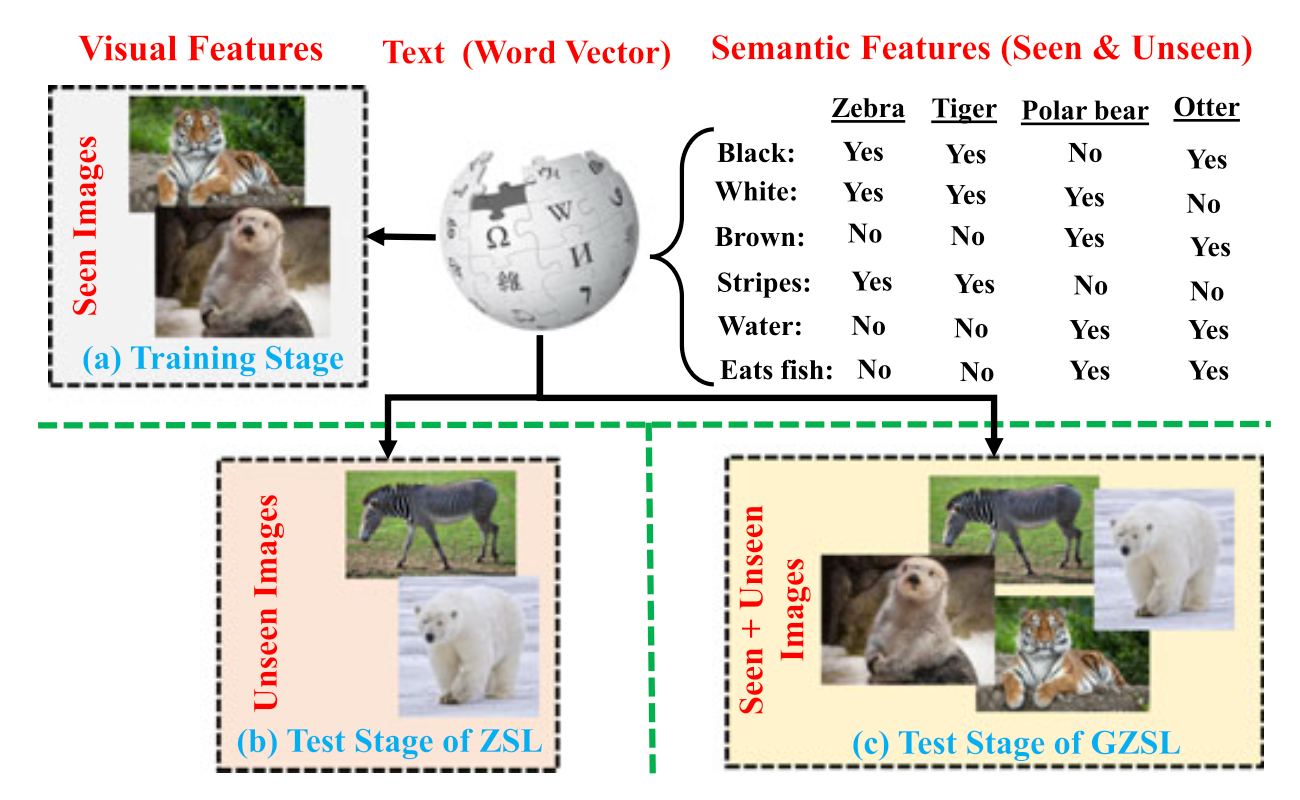
\includegraphics[width=1.0\textwidth]{figures/zsl_framework.png}
\caption{零样本学习基本框架示意图\cite{pourpanah2023review}}
\label{fig:zsl_framework}
\end{figure}

形式化地，设已见类别集合为$\mathcal{Y}_s$，未见类别集合为$\mathcal{Y}_u$，且$\mathcal{Y}_s \cap \mathcal{Y}_u = \varnothing$。训练集$\mathcal{D}_s = \{(\mathbf{x}_i, y_i)\}_{i=1}^{N_s}$仅包含属于$\mathcal{Y}_s$的标注样本。每个类别$y$对应一个语义描述向量$\mathbf{a}_y \in \mathbb{R}^{d_a}$，该向量可以来自人工定义的属性、词向量或预训练语言模型编码的文本嵌入。零样本学习的目标是学习映射函数$f: \mathcal{X} \to \mathcal{A}$，将样本特征映射至语义空间，使得在推理阶段可通过语义匹配完成对未见类别的分类，如公式~\eqref{eq:zsl_mapping}和公式~\eqref{eq:zsl_inference}所示：
\begin{equation}
\label{eq:zsl_mapping}
f: \mathcal{X} \to \mathcal{A}
\end{equation}
\begin{equation}
\label{eq:zsl_inference}
\hat{y} = \arg\max_{y \in \mathcal{Y}_u} \text{sim}(f(\mathbf{x}), \mathbf{a}_y)
\end{equation}
其中$\text{sim}(\cdot, \cdot)$为相似度函数（如余弦相似度或点积）。在更具挑战性的广义零样本学习（Generalized Zero-Shot Learning, GZSL）设定下，测试阶段的候选类别同时包含已见和未见类别$\mathcal{Y}_s \cup \mathcal{Y}_u$，模型不仅需要识别未见类别，还需保持对已见类别的判别能力。

\subsection{嵌入空间对齐机制}

零样本学习的核心技术问题在于如何构建高质量的跨模态映射，使得样本特征与类别语义描述在共享嵌入空间中实现有效对齐。根据映射方向的不同，现有方法可分为三种范式。

第一种是从特征空间到语义空间的前向映射。设样本特征为$\mathbf{x} \in \mathbb{R}^{d_x}$，语义描述为$\mathbf{a}_y \in \mathbb{R}^{d_a}$，该范式学习映射$f_\theta: \mathbb{R}^{d_x} \to \mathbb{R}^{d_a}$，通过最小化如公式~\eqref{eq:zsl_forward}所示的对齐损失实现映射学习：
\begin{equation}
\label{eq:zsl_forward}
\mathcal{L}_{align} = \sum_{i=1}^{N_s} \ell(f_\theta(\mathbf{x}_i), \mathbf{a}_{y_i})
\end{equation}
其中$\ell(\cdot, \cdot)$为距离度量函数。该方法实现简洁，但由于训练仅使用已见类别数据，所学映射在未见类别的语义区域可能不够准确，这一问题称为域偏移（Domain Shift）\cite{pourpanah2023review}。

第二种是双向映射范式，同时学习从特征空间到语义空间以及从语义空间到特征空间的双向映射，并通过重建约束缓解信息丢失。具体而言，编码器$f_\theta$将样本映射至语义空间，解码器$g_\phi$将语义表示重建回特征空间，总损失函数如公式~\eqref{eq:zsl_bidir}所示：
\begin{equation}
\label{eq:zsl_bidir}
\mathcal{L}_{bidir} = \sum_{i=1}^{N_s} \left[\ell(f_\theta(\mathbf{x}_i), \mathbf{a}_{y_i}) + \lambda \|\mathbf{x}_i - g_\phi(f_\theta(\mathbf{x}_i))\|^2\right]
\end{equation}
其中$\lambda$为重建损失的权重系数。SAE（Semantic Autoencoder）\cite{kodirov2017semantic}是该范式的代表性方法，通过编码器—解码器结构约束映射的双向一致性。

第三种是共享嵌入空间范式，将样本特征和语义描述分别通过各自的投影网络映射至同一低维空间，如公式~\eqref{eq:zsl_shared}所示：
\begin{equation}
\label{eq:zsl_shared}
\mathbf{z}_x = \phi_x(\mathbf{x}), \quad \mathbf{z}_a = \phi_a(\mathbf{a}_y)
\end{equation}
其中$\phi_x$和$\phi_a$分别为特征投影网络和语义投影网络，训练目标是使正样本对$(\mathbf{z}_x, \mathbf{z}_a)$在嵌入空间中距离最近。该范式的优势在于两种模态共同适配至对等的嵌入空间，避免了单向映射的不对称偏差。CLIP\cite{radford2021learning}通过在大规模图像—文本对上进行对比学习预训练，是该范式最具代表性的工作，仅需输入类别名称或文本描述便可直接完成零样本分类。本论文第三章的MZSGO正是采用共享嵌入空间范式，将蛋白质特征与GO功能语义投影至统一隐空间进行匹配。

\subsection{基于对比学习的语义匹配}

在共享嵌入空间范式下，对比学习是实现跨模态语义对齐的核心训练机制。其基本思想是：在一批训练样本中，将匹配的样本-语义对（正样本对）在嵌入空间中拉近，同时将不匹配的对（负样本对）推远。InfoNCE\cite{oord2018representation}损失函数是对比学习中最具代表性的优化目标，给定一批$B$个样本，其形式化定义如公式~\eqref{eq:infonce_zsl}所示：
\begin{equation}
\label{eq:infonce_zsl}
\mathcal{L}_{CL} = -\frac{1}{B}\sum_{i=1}^{B}\log\frac{\exp(\text{sim}(\mathbf{z}_x^i, \mathbf{z}_a^i)/\tau)}{\sum_{j=1}^{B}\exp(\text{sim}(\mathbf{z}_x^i, \mathbf{z}_a^j)/\tau)}
\end{equation}
其中$\mathbf{z}_x^i$和$\mathbf{z}_a^i$分别为第$i$个样本的特征投影和对应类别的语义投影，$\text{sim}(\cdot, \cdot)$为余弦相似度，$\tau$为温度超参数。温度参数$\tau$控制分布的集中程度：$\tau$较小时，损失函数对困难负样本（与正样本对语义接近的负样本）赋予更大的梯度权重，有利于学习细粒度的语义区分；$\tau$较大时则使梯度分布更为平滑。

对比学习实现零样本推断的关键在于：当嵌入空间中的语义对齐足够充分时，即使某个类别的语义描述$\mathbf{a}_{y_u}$在训练阶段从未作为正样本出现过，只要其语义投影$\mathbf{z}_{a}^{y_u}$与测试样本的特征投影$\mathbf{z}_{x}$在嵌入空间中距离较近，模型便能基于这种语义邻近性做出正确预测。这一特性使得对比学习天然适用于开放标签空间的零样本预测任务。

在语义描述的构建方面，语义空间的表达质量直接制约零样本学习的性能上界。早期方法依赖人工定义的属性向量\cite{lampert2014attribute}，语义粒度有限且构建成本高昂；随后发展到利用词向量（如Word2Vec\cite{mikolov2013efficient}、GloVe\cite{pennington2014glove}）编码类别名称，能够自动捕获词汇间的语义关系，但仅编码了表层语义；当前最先进的方法使用预训练语言模型（如BERT\cite{devlin2019bert}）或大语言模型对类别的完整文本定义进行编码，能够捕获深层语义信息和上下文关联，显著提升了语义空间的表达能力。

在蛋白质功能预测中，GO术语具有标准化的文本名称和详细的功能定义，利用高质量预训练语言模型对这些文本进行编码，能够构建语义丰富且结构化的功能标签嵌入空间。本论文第三章正是借鉴上述对比学习的嵌入对齐思想和基于文本的语义空间构建方法，将蛋白质功能预测重构为蛋白质特征与GO功能语义之间的匹配问题，以实现对未见功能标签的零样本推断。

\section{预训练技术相关研究}

预训练技术通过在大规模无标注数据上进行自监督学习赋予模型通用的表示能力，已成为当前蛋白质功能预测方法的重要基础。本节从预训练技术的一般框架出发，系统梳理语言模型预训练、蛋白质语言模型、多模态预训练以及参数高效微调与知识蒸馏等方面的技术发展。

\subsection{语言模型预训练的发展}

语言模型预训练是当前深度学习中最重要的技术范式之一，其核心思想是在大规模无标注文本上进行自监督训练以学习通用语言表示，再通过微调迁移至下游任务，这一范式的成功为蛋白质语言模型的发展奠定了基础。

\begin{figure}[htbp]
\centering
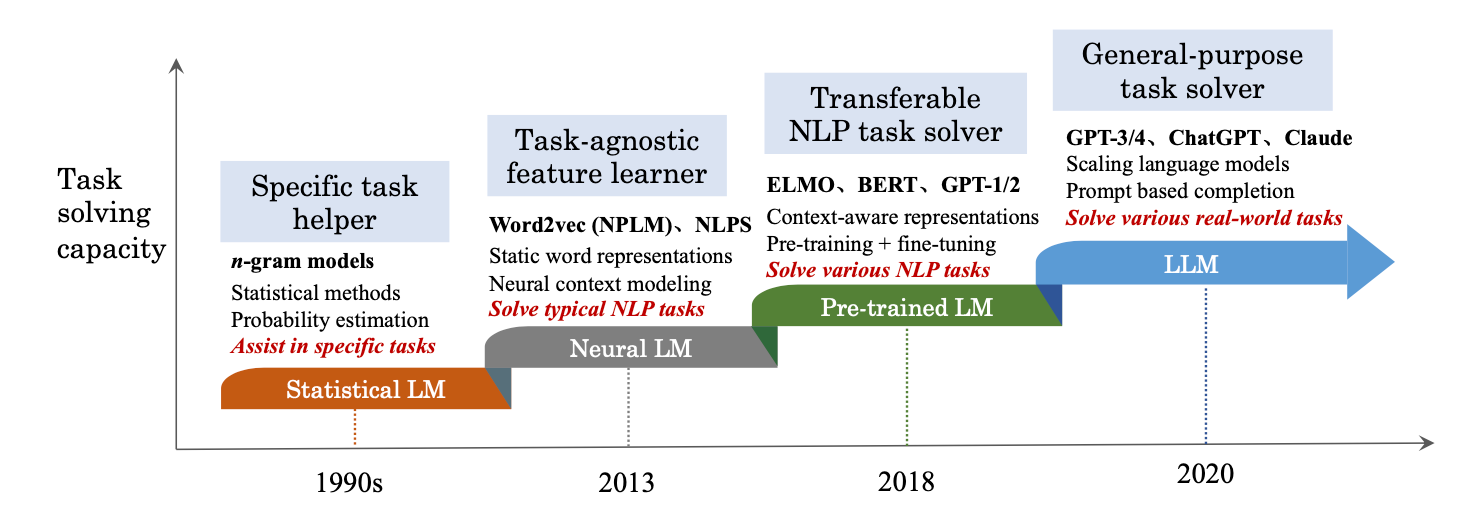
\includegraphics[width=1.0\textwidth]{figures/lm_evolution.png}
\caption{语言模型预训练技术的发展历程\cite{zhao2023survey}}
\label{fig:lm_evolution}
\end{figure}

如图~\ref{fig:lm_evolution}所示，语言模型预训练经历了从静态词向量到大语言模型的演进。Word2Vec\cite{mikolov2013efficient}和GloVe\cite{pennington2014glove}为每个词学习固定的稠密向量，捕捉了词汇间语义关系但无法处理一词多义。ELMo\cite{peters2018deep}通过双向LSTM生成上下文敏感的动态词嵌入。

Transformer架构\cite{vaswani2017attention}的提出是语言模型发展的里程碑。该架构完全基于自注意力（Self-Attention）机制，通过缩放点积注意力实现对序列中任意位置之间依赖关系的直接建模，如公式~\eqref{eq:attention}所示：
\begin{equation}
\label{eq:attention}
\text{Attention}(\mathbf{Q}, \mathbf{K}, \mathbf{V}) = \text{softmax}\left(\frac{\mathbf{Q}\mathbf{K}^\top}{\sqrt{d_k}}\right)\mathbf{V}
\end{equation}
其中$\mathbf{Q}$、$\mathbf{K}$、$\mathbf{V}$分别为查询、键和值矩阵，$d_k$为键向量的维度。多头注意力机制进一步将输入投影到$h$个不同的子空间中并行计算，增强了模型对多层次依赖关系的捕获能力。

基于Transformer架构，BERT\cite{devlin2019bert}采用掩码语言建模（Masked Language Modeling, MLM）目标进行双向预训练，通过预测被随机遮掩的词来学习深层上下文表示。GPT系列模型\cite{radford2019language}则采用自回归语言建模目标，通过预测下一个词来学习序列生成能力。这两种预训练范式分别代表了编码器和解码器两条技术路线：MLM更适合需要全局上下文理解的判别式任务，自回归建模则更适合文本生成任务。

近年来，随着模型规模的持续扩大，大语言模型展现出"涌现能力"（Emergent Abilities），推动了从通用语言模型到领域专用语言模型的发展，蛋白质语言模型正是这一趋势在生物学领域的重要体现。

\subsection{蛋白质语言模型}

蛋白质序列与自然语言之间存在深刻的结构类比：20种标准氨基酸构成"词汇表"，氨基酸序列构成"语句"，序列中氨基酸间的共进化关系类似于语言中的语法和语义依赖，这为语言模型预训练技术向蛋白质领域的迁移提供了理论基础。

蛋白质语言模型的发展经历了从浅层模型到深层Transformer模型的演进。早期的UniRep\cite{alley2019unified}和SeqVec\cite{heinzinger2019modeling}分别采用多层LSTM和双向LSTM学习蛋白质序列表示，验证了自监督语言建模在蛋白质序列上的可行性。随后，基于Transformer架构的ProtBert\cite{elnaggar2022prottrans}和ProtTrans系列\cite{elnaggar2022prottrans}将BERT和T5的预训练范式直接应用于蛋白质序列。ESM-1b\cite{rives2021biological}证明了蛋白质语言模型性能随参数规模增长而持续提升。ESM-2\cite{lin2023evolutionary}是目前最具代表性的蛋白质语言模型之一，如图~\ref{fig:esm2}所示，其核心训练目标为掩码语言建模。

\begin{figure}[htbp]
\centering
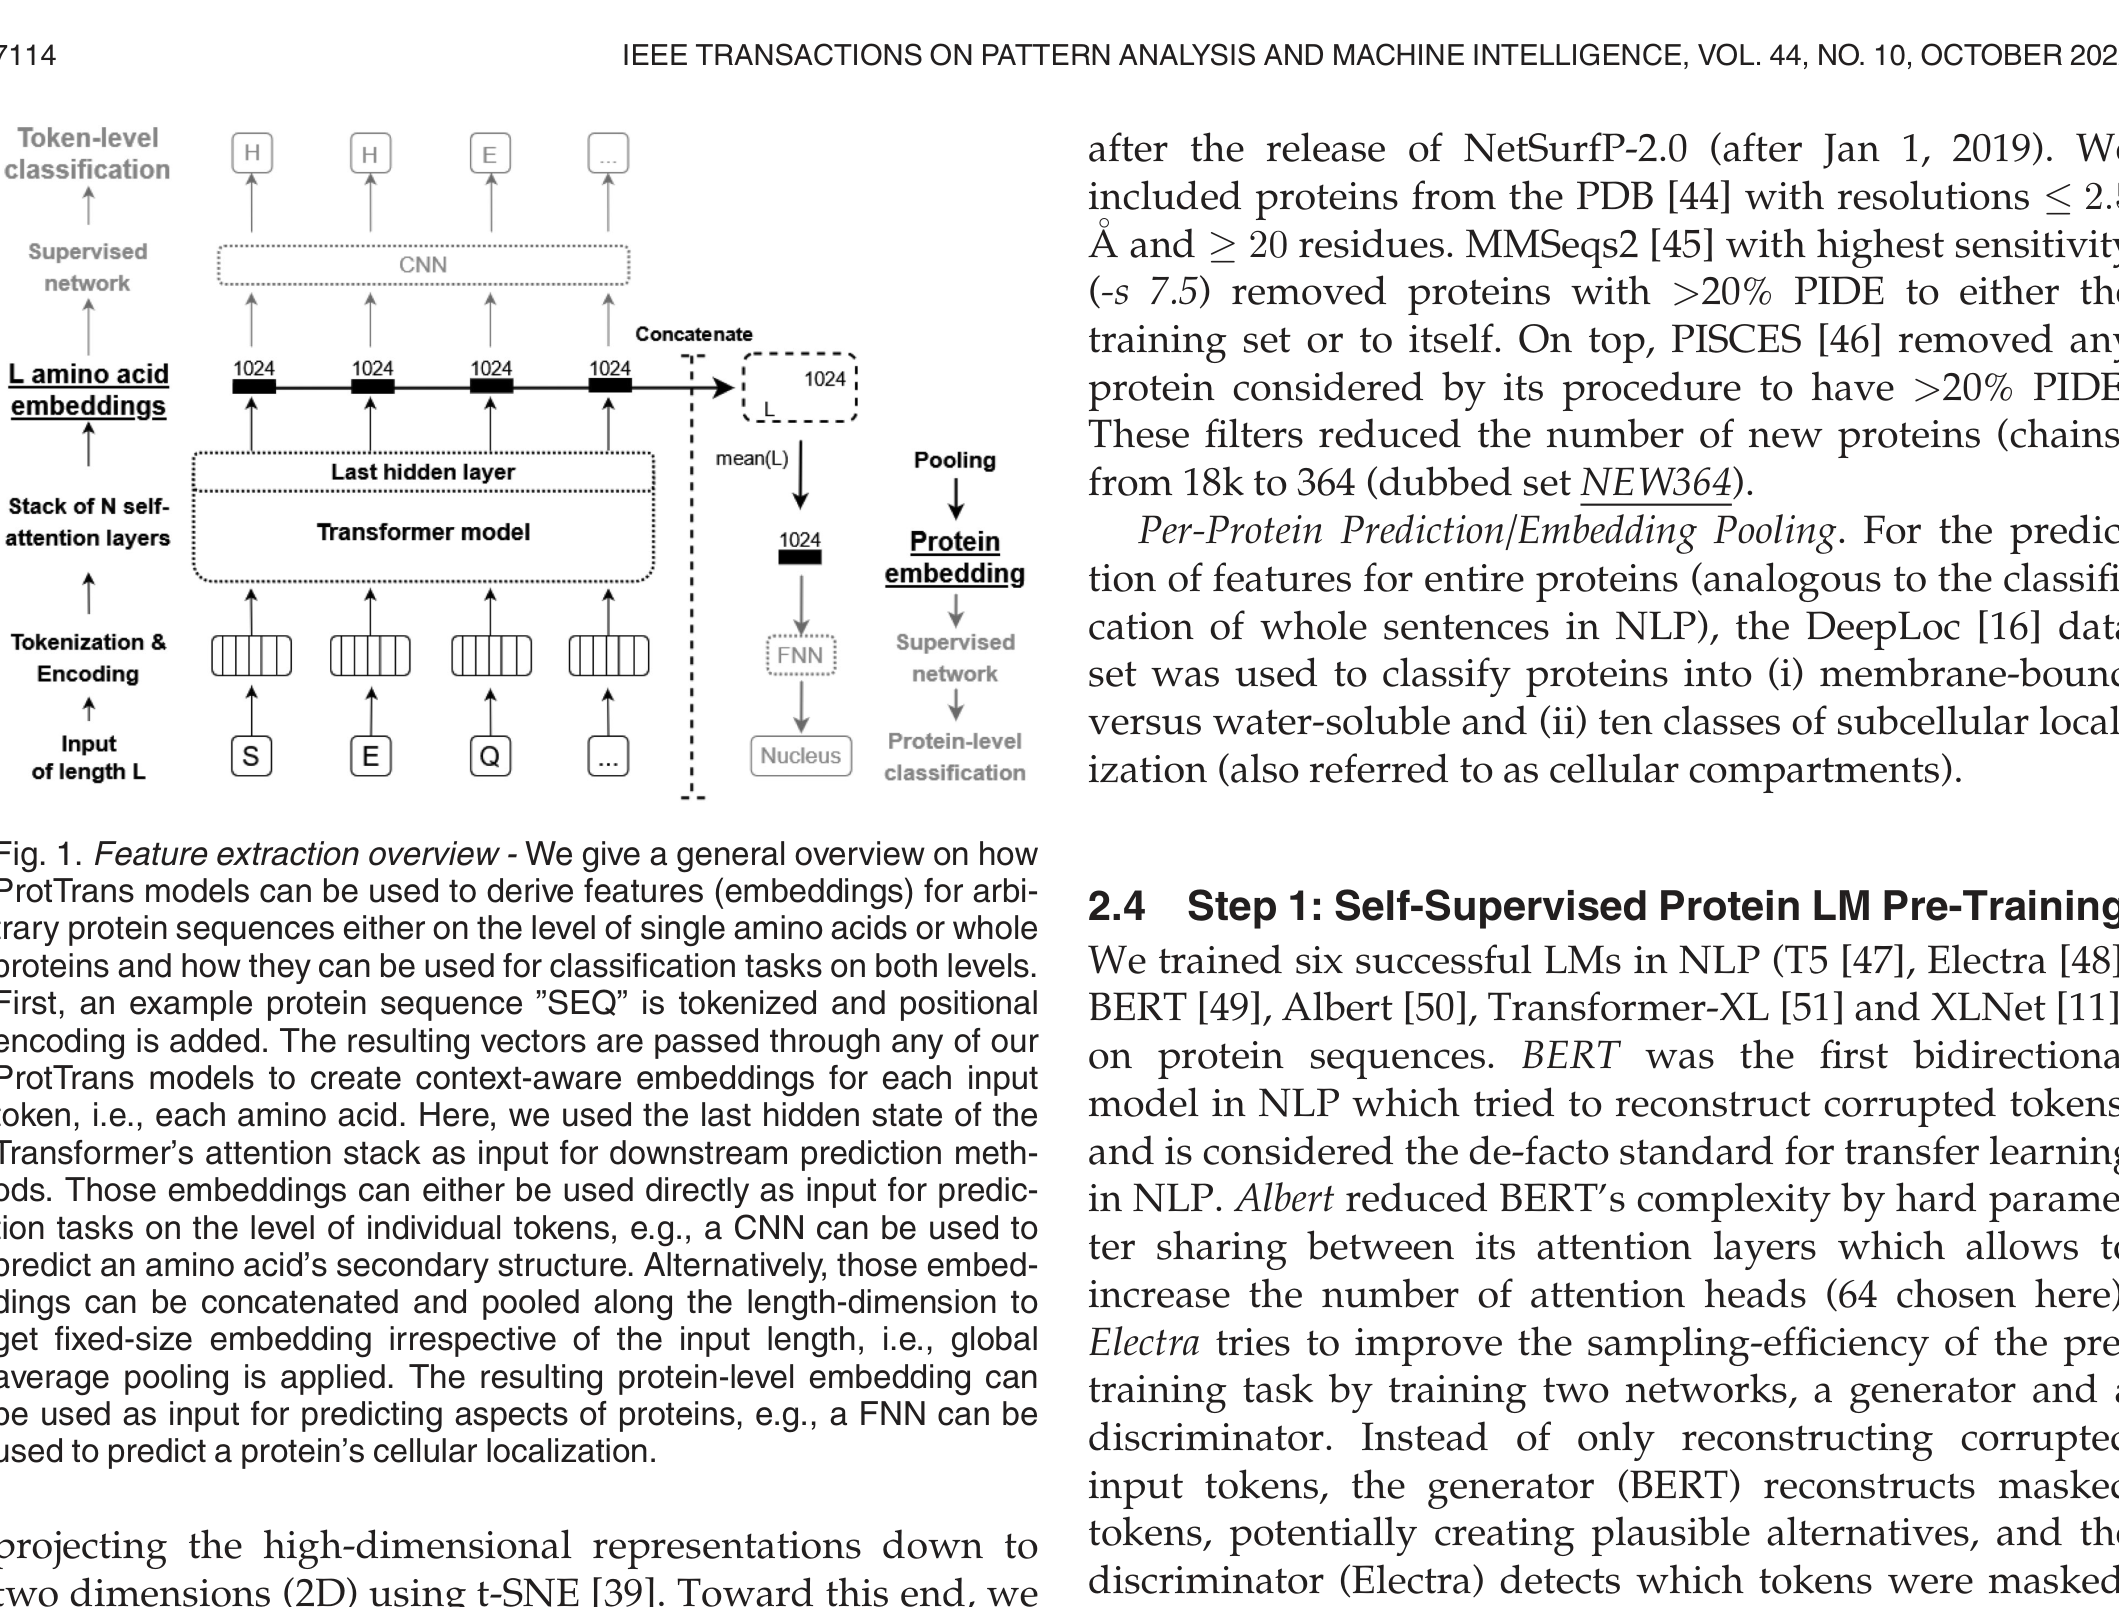
\includegraphics[width=1.0\textwidth]{figures/esm2.png}
\caption{蛋白质语言模型预训练与特征提取示意图\cite{elnaggar2022prottrans}}
\label{fig:esm2}
\end{figure}

ESM-2在输入序列中随机遮掩一定比例的氨基酸位置，模型需根据上下文信息预测被遮掩的氨基酸。设蛋白质序列为$\mathbf{s} = (s_1, s_2, \ldots, s_L)$，遮掩位置集合为$\mathcal{M}$，则MLM的训练目标为：
\begin{equation}
\mathcal{L}_{\text{MLM}} = -\sum_{j \in \mathcal{M}} \log p(s_j \mid \mathbf{s}_{\setminus \mathcal{M}})
\end{equation}
其中$\mathbf{s}_{\setminus \mathcal{M}}$表示未被遮掩的序列部分。通过在UniRef数据库约2.5亿条序列上训练，ESM-2能够隐式编码氨基酸的共进化模式、接触关系和保守性特征。ESM-2采用标准Transformer编码器架构，具有从800万到150亿参数的多个规模变体。

蛋白质语言模型的成功表明，自监督预训练能够从序列数据中学到有意义的生物学特征，这些预训练表示已成为当前多数蛋白质功能预测方法的基础编码器。

\subsection{多模态预训练}

单模态预训练虽然在各自领域取得了显著成效，但蛋白质的功能特性往往需要结合序列、结构、文本等多种信息才能全面刻画。多模态预训练旨在联合学习不同模态间的对应关系以构建更具表达力的统一表示。CLIP\cite{radford2021learning}通过大规模图像-文本对比学习证明了跨模态对齐预训练的有效性，如图~\ref{fig:contrastive}所示，对比学习通过正负样本对的构造实现跨模态语义对齐。

\begin{figure}[htbp]
\centering
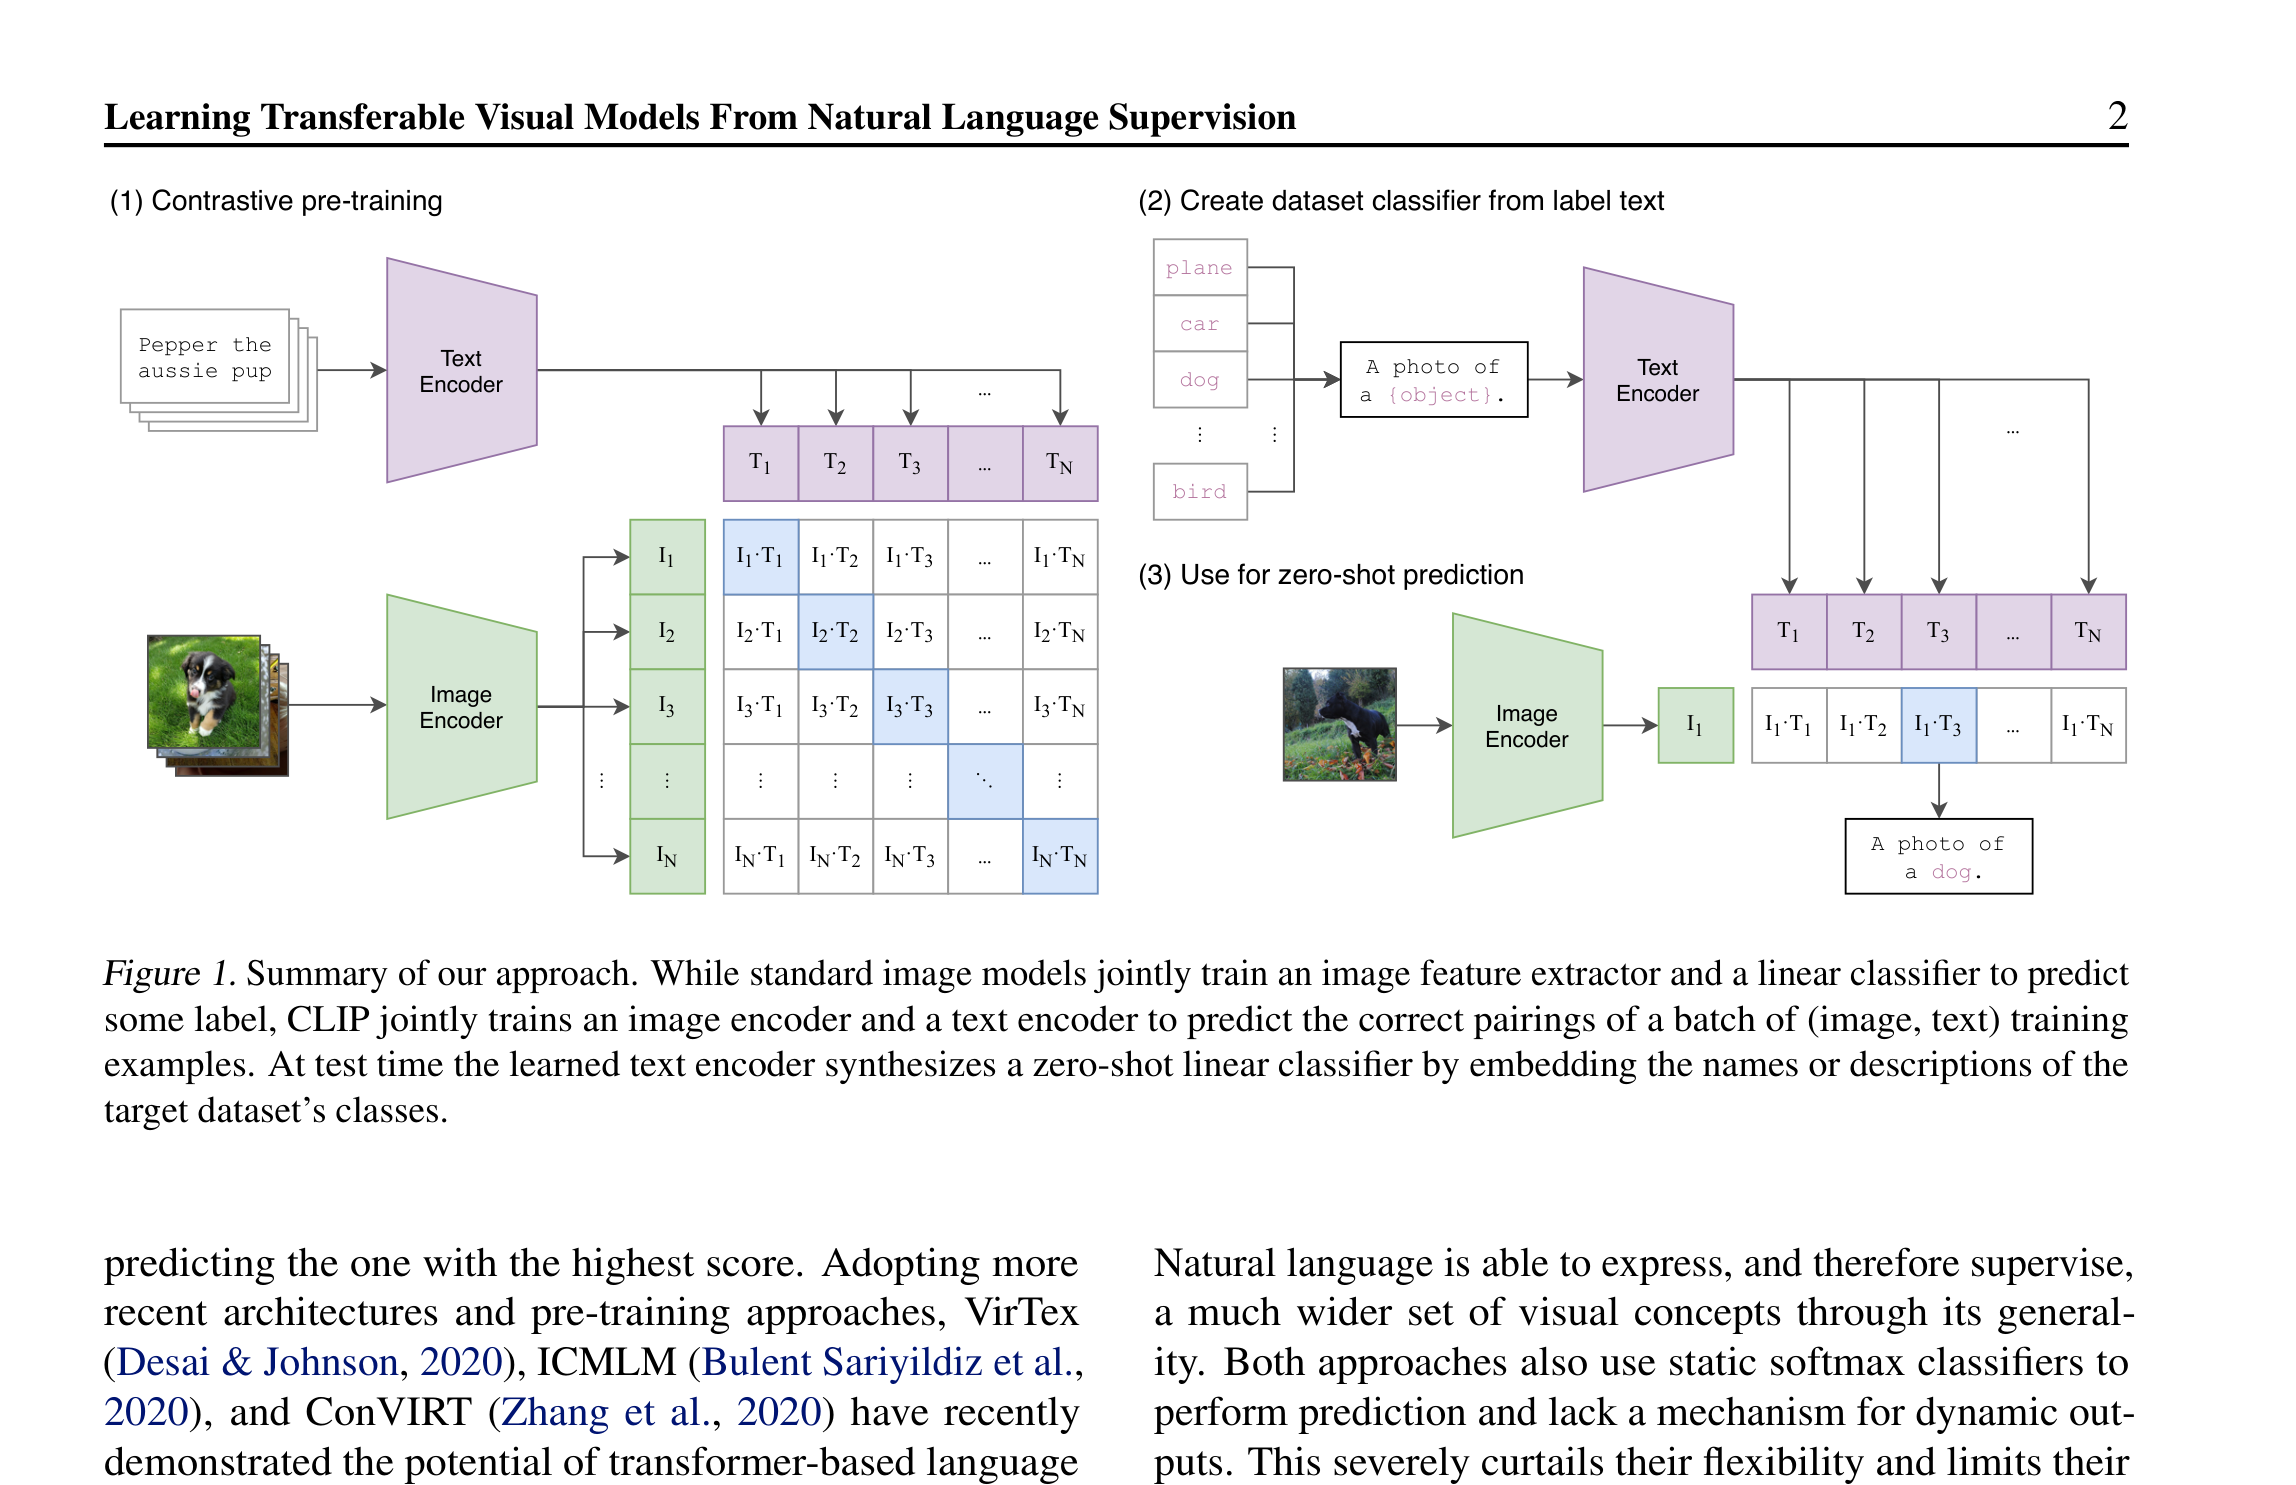
\includegraphics[width=1.0\textwidth]{figures/contrastive.png}
\caption{基于对比学习的多模态预训练示意图\cite{radford2021learning}}
\label{fig:contrastive}
\end{figure}

InfoNCE\cite{oord2018representation}损失函数是对比学习中最具代表性的优化目标。给定一批$B$个样本，每个样本$i$对应两种模态的表示$\mathbf{z}_i^A$和$\mathbf{z}_i^B$，损失如公式~\eqref{eq:infonce}所示：
\begin{equation}
\label{eq:infonce}
\mathcal{L}_{\text{InfoNCE}} = -\frac{1}{B}\sum_{i=1}^{B}\log\frac{\exp(\text{sim}(\mathbf{z}_i^A, \mathbf{z}_i^B)/\tau)}{\sum_{j=1}^{B}\exp(\text{sim}(\mathbf{z}_i^A, \mathbf{z}_j^B)/\tau)}
\end{equation}
其中$\text{sim}(\cdot, \cdot)$为余弦相似度，$\tau$为温度超参数，控制分布的集中程度。

在蛋白质领域，多模态预训练沿两条路线发展：一是知识增强预训练，将GO本体结构、知识图谱和生物医学文本等外部知识融入预训练过程；二是结构-序列联合预训练，如S-PLM\cite{wang2025splm}通过适配器模块和对比学习将结构信息蒸馏至序列表示中，使模型仅凭序列输入即可获得结构感知表示。这一趋势为本论文第四章的域感知适配器预训练提供了直接的技术启发。

\subsection{参数高效微调与知识蒸馏}

大规模预训练模型（如ESM2-650M）包含数亿参数，全参数微调不仅计算成本高昂，还易导致灾难性遗忘。参数高效微调（Parameter-Efficient Fine-Tuning, PEFT）技术通过冻结原始参数、仅训练少量额外参数来适配下游任务。根据参数引入方式，PEFT方法主要分为三类。第一类是适配器方法（Adapter）\cite{houlsby2019adapter}，在每层中插入轻量级瓶颈结构模块。如图~\ref{fig:adapter}所示，适配器通过降维—激活—升维的瓶颈结构与残差连接实现任务适配，如公式~\eqref{eq:adapter_ch2}所示：
\begin{equation}
\label{eq:adapter_ch2}
\text{Adapter}(\mathbf{x}) = \mathbf{W}_{up} \cdot \sigma(\mathbf{W}_{down} \cdot \mathbf{x}) + \mathbf{x}
\end{equation}
其中$\mathbf{W}_{down} \in \mathbb{R}^{d_b \times d}$为降维矩阵，$\mathbf{W}_{up} \in \mathbb{R}^{d \times d_b}$为升维矩阵，$d_b \ll d$为瓶颈维度。

\begin{figure}[htbp]
\centering
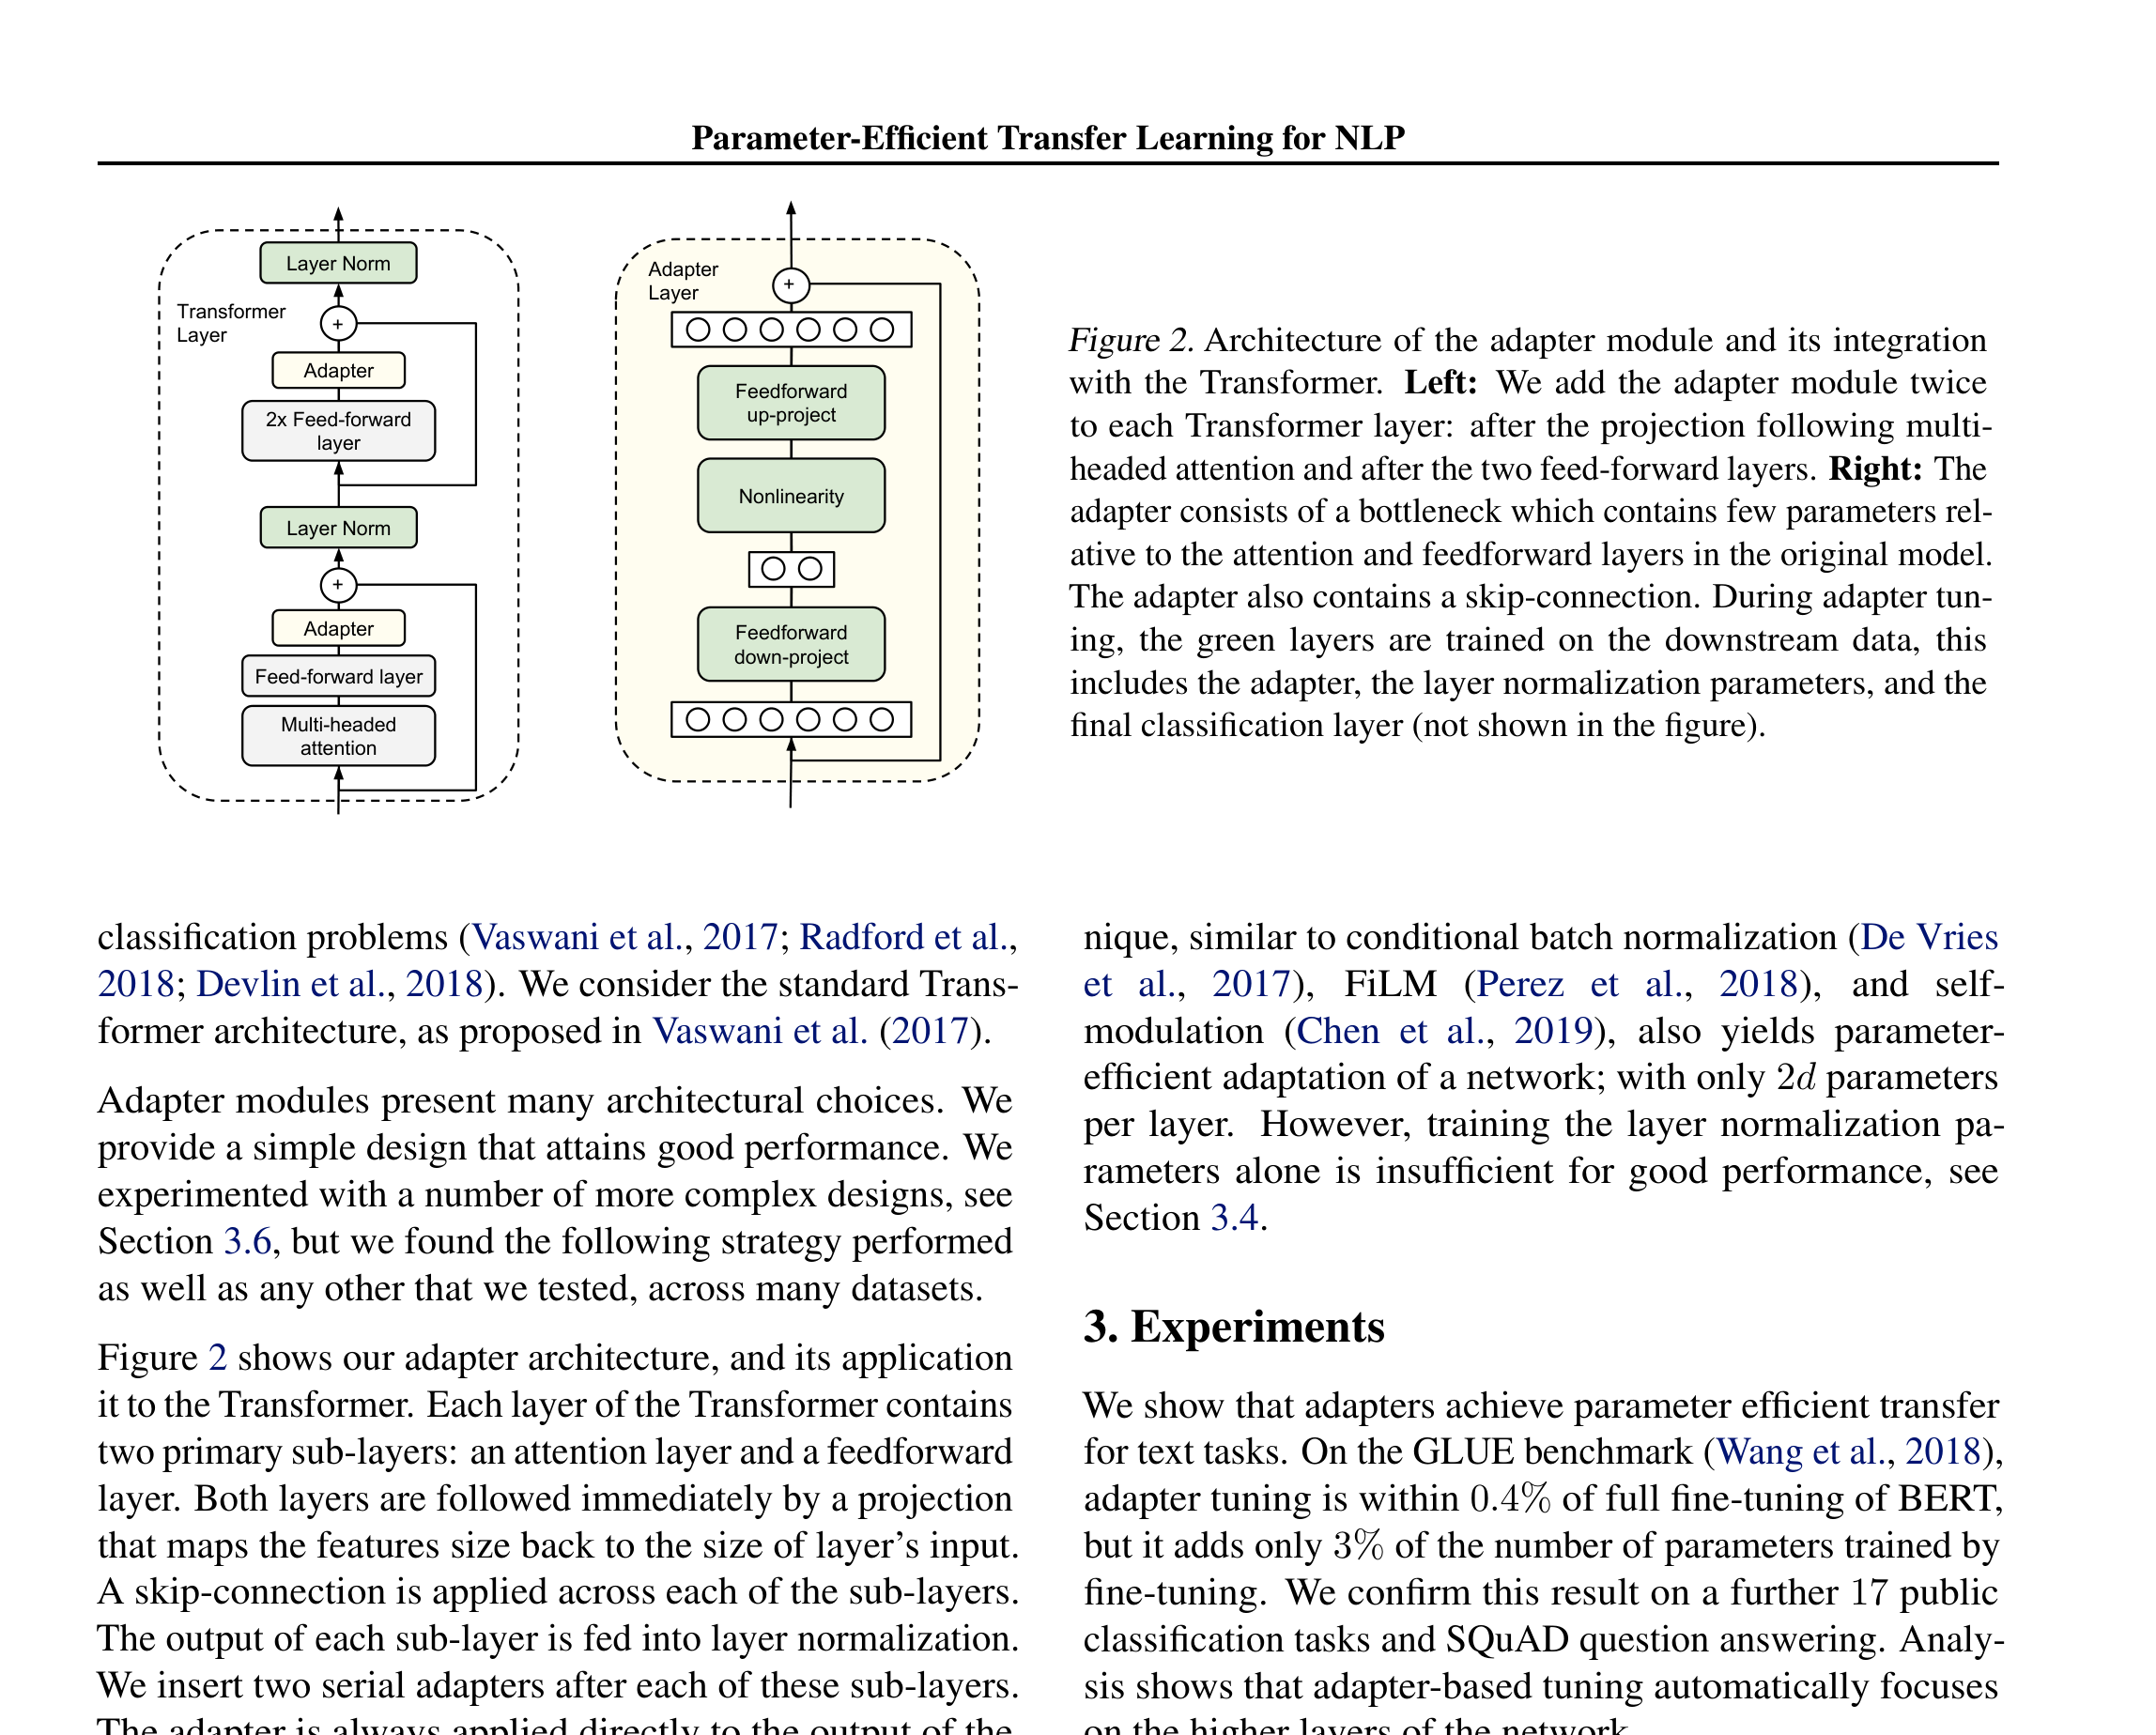
\includegraphics[width=1.0\textwidth]{figures/adapter.png}
\caption{适配器与参数高效微调示意图\cite{houlsby2019adapter}}
\label{fig:adapter}
\end{figure}

第二类是提示微调方法（Prompt Tuning），通过在输入序列前添加可学习的连续提示向量来引导模型适配特定任务，无需修改模型内部结构。第三类是低秩适配方法（LoRA）\cite{hu2022lora}，通过低秩分解对模型权重矩阵进行增量更新。这些方法各有特点，适配器方法因其结构清晰、易于与跨模态蒸馏结合而在蛋白质领域得到较多应用。

知识蒸馏（Knowledge Distillation）\cite{hinton2015distilling}是另一项与参数高效微调密切相关的技术。最初提出时，知识蒸馏用于模型压缩，让小型学生模型学习大型教师模型的输出分布，如公式~\eqref{eq:kd_loss}所示：
\begin{equation}
\label{eq:kd_loss}
\mathcal{L}_{\text{KD}} = T^2 \cdot \text{KL}\left(\text{softmax}\left(\frac{\mathbf{z}_T}{T}\right) \middle\| \text{softmax}\left(\frac{\mathbf{z}_S}{T}\right)\right)
\end{equation}
其中$\mathbf{z}_T$和$\mathbf{z}_S$分别为教师和学生模型的输出logits，$T$为蒸馏温度。

在更广义的框架下，知识蒸馏可理解为跨模态知识转移机制。这一思想与PEFT的结合催生了一条重要技术路线：利用适配器作为蒸馏载体，将跨模态知识蒸馏至轻量级参数中，既保留预训练模型的通用表示又注入领域知识。S-PLM\cite{wang2025splm}正是这一路线的代表，通过对比学习将结构信息蒸馏至ESM-2适配器参数中。本论文第四章进一步将蒸馏目标拓展为域功能语义信息，并设计双适配器策略以平衡预训练知识保留与下游任务优化。

\section{本章小结}

本章围绕蛋白质功能预测所需的前序知识进行了系统介绍。首先从任务层面对蛋白质功能预测问题进行了形式化定义，介绍了GO层级体系、多标签预测特性、广义零样本设定以及开放标签空间下的"蛋白质—功能"语义匹配建模思路，并总结了$F_{\max}$、AUPR和调和均值$H$等常用评价指标。

随后，介绍了零样本学习的形式化定义与核心技术机制，从前向映射、双向映射到共享嵌入空间三种范式详细阐述了嵌入空间对齐的技术原理，并介绍了基于对比学习的语义匹配方法及语义空间构建策略，为后续将蛋白质功能预测建模为语义匹配问题奠定了方法论基础。之后，系统介绍了预训练技术的基本原理，涵盖语言模型预训练、蛋白质语言模型、多模态预训练以及参数高效微调与知识蒸馏等关键方向。

本章介绍的各项技术构成了后续研究的理论基础。其中，蛋白质语言模型提供底座表征能力，零样本学习框架为开放标签预测提供方法论支撑，多模态预训练为跨模态语义注入提供技术手段，参数高效微调为低成本适配下游任务提供实现路径。基于上述分析，本论文后续将分别从开放标签语义匹配建模（第三章）和参数高效预训练增强（第四章）两个方向展开方法研究。
